\chapter{Introduction}
\section{Background and problem motivation}
The research department for computer vision at mid Sweden university (MIUN) uses multiple Raspberry PIs to capture threedimensional data. Because recalibration of multi camera systems is computationally intensive and the computational resources of the hardware is limited, unnecessary recalculations should be avoided. If the camera positions do not change over time, no recalibration is required. Therefore, an algorithm which is capable of determining camera movement solely from the videostream could abandon the need for interval recalibrations without the need of additional sensors.

\section{Scope}
The main focus of this project lies in distinguishing between changes of the camera itself and changes in the scene. Furthermore, the resulting algorithm should easily be integratable into a gstreamer-application, which is used in the research departement for computer vision at MIUN. This project should give an example on how halide can be used within gstreamer on an embedded plattforms.

The effects of environmental differences is not covered in this project but only assumptions by the author are given in the outlook for further investigations.

\section{Goals}
\begin{tabular}{|l|p{13cm}|}
	\hline G1 & false negative rate have to be below 5\% \\ 	
	\hline G2 & false positive rate have to be bellow 1\% \\ 	
	\hline G3 & The software should run on the raspberry pi hardware \\
	\hline 
\end{tabular} 
$$ G1= \mathit{falseNegatives} / \mathit{numberOfExpectedChanges} $$
$$ G2= \mathit{falsePositives} / \mathit{numberOfFrames} $$

Although a low $\mathit{false negative}$ rate is much more important than a low $\mathit{falsePositives}$ rate, the boundaries of G1 are narrower than G2's. This is reasoned by the fact that $\mathit{numberOfFrames} \gg \mathit{numberOfExpectedChanges}.$

\chapter{Theory}
 \section{ Harris}
 \label{sec:harris}
In order to find distinctive points within an image, a corner detection could be applied to the input image. Compared to simple Edge-Filters as Sobel or Prewitt, Harris finds corners where edges detected by Prewitt- or Sobelfilters are ending or crossing each other \cite{edge-detection}. Therefore, after a movement of the camera in any directions, the corner will not be found at the same position again, whereas a point representing an edge would still find an edge if the camera moves along its direction.  \newline

Unfortunately, the approach to find the center of corners with local maximum does not assure a good distribution of the results accross the image \cite{harris-detector}. If just the n most distinctive pixels are selected, they might all be in the same region of the image and a moveing object in the scene might cover them all at the same time.

\section{Type casting}
As shown in listing 1, C doesn't handle overflows consistently. Even thought it is a 64 Bit System, which was determined by printing sizeof($int^*$), overflows in uint8\_t were preserved on shift back whereas uint32\_t looses this information. Even thought this project might benefit from using 8bit calculations, 8 bit values are casted to 16 bit before a calculation when the intermediate results could exceed 255 to assure a portable and stable solution.

\begin{listing}[]
	
	\begin{minted}[linenos=true]{cpp}
	#include <stdio.h>
	#include <stdint.h>
	#include <limits.h>
	
	int main()
	{
	uint32_t a = UULONG_MAX>>32,
	b = UULONG_MAX>>32,
	res = (uint32_t)((a+b)>>1);
	printf("Result(%lu): %lu\n", a, res);
	
	return 0;
	}
	\end{minted}
	\textit{ Result (4294967295): 2147483647 \\
		(2\textsuperscript{32}-1): (2\textsuperscript{31}-1)
	}
	\begin{minted}[linenos=true]{cpp}
	#include <stdio.h>
	#include <stdint.h>
	#include <limits.h>
	
	int main()
	{
	uint8_t a = 255,
	b = 255,
	res = (uint8_t)((a+b)>>1);
	printf("Result(%u): %u\n", a,res);
	
	return 0;
	}
	
	\end{minted}
	\label{alg:the-code}
	\caption{Compare 8bit vs. 32bit overflow}
	\textit{ Result(255): 255 }
\end{listing}
To assure repeatability, this demonstration was executed on \\ https://www.tutorialspoint.com/compile\_c\_online.php.


\chapter{ Methology}
\section{Capturing}

In order to get meaningful video-testdata it is important to record uncompressed data to avoid changeing the imagedata. For that task, the library picamera:1.12 was used which has the ability to record uncompressed yuv data \cite{rawrecording}. Unfortunately, this requires a big bandwidth. 

\subsection{Minimal requirements}
\begin{description}
	\item[Resolution] 1280x720px
	\item[Framerate] 10fps
	\item[Viewport] Full Area
\end{description}
Recordings in YUV color format, which uses 1.5 bytes per pixel, results in
$$10 * 1280 * 720 * 1.5 = 13.2 MB/s$$

Tests with the software sdbench.sh \cite{sdbench}, showed, that the Raspbian SD-card wasn't able to meet this requirement, because it's maximum  bandwidth was just about 10MB/s. (\enquote{drivespeed.xlsx}). Unfortunately this was not indicated by an error but led to missing frame in the resulting file.

Therefore, a \enquote{TOSHIBA EXCERIA XC 64GB} was used for further recordings, which, according to sdbench.sh, can handle framerates up to 15.55 MB/s on the Raspberry pi.

\subsection{Ring-byte-buffer}
Even thought the bandwidth was theoretically big enough, there were still missing frames. Therefore, a byte-ring-buffer was implemented to record into RAM directly (fig. 4.2). The fact that a separate thread is constantly writing this Buffer into a file, has three advantages:
\begin{description}
	\item[Constant writing] No SD-card bandwidth is wasted during frame capturing. The separate thread is constantly writing.
	\item[Shortterm increased Bandwidth] Because of the buffer, which might be several hundred MB in size, the recording bandwidth can exceed the SD-Card bandwith for short recordings.
	\item[Error on failure] If the ring-buffer is full, an exception is raised and frames are not silently dropped anymore.
\end{description}

\begin{figure}[h!]
	\centering
	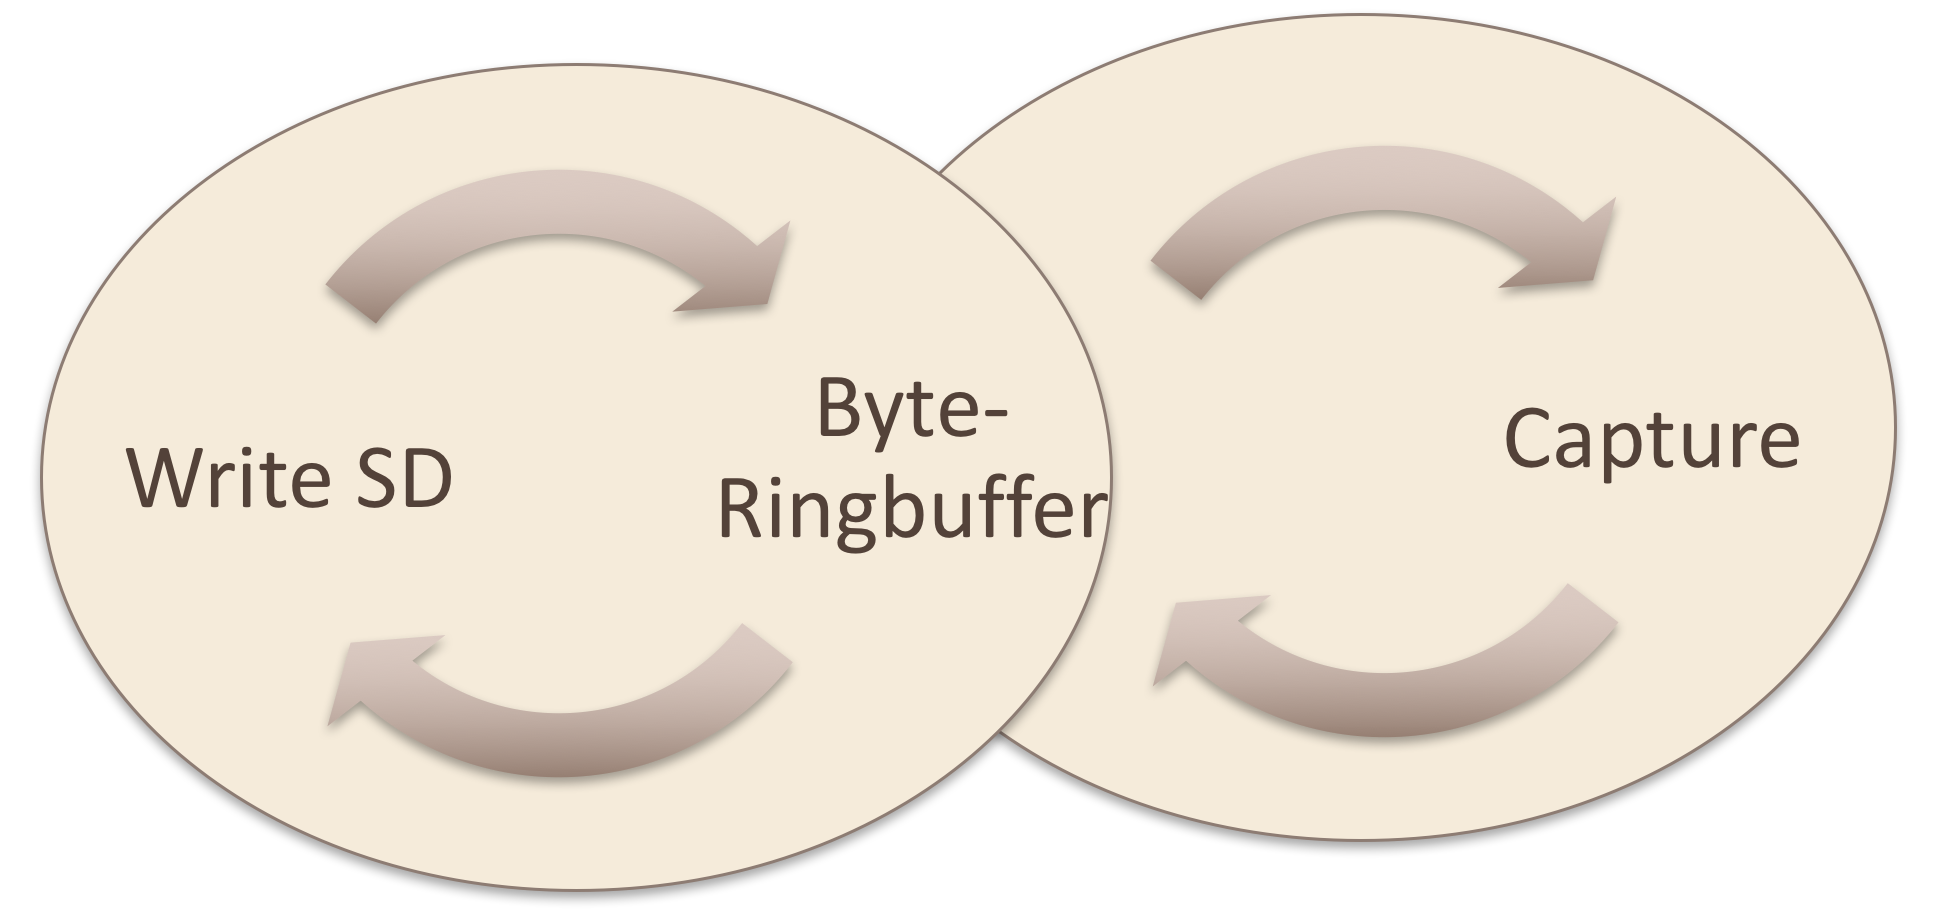
\includegraphics[width=0.9\linewidth]{bin/ringbuffer}
	\caption{Each arrow ring represents a working thread. }
	\label{fig:ringbuffer}
\end{figure} 

\section{Evaluation}
\label{sec:sequences}
In order to compare the results of different algorithms, 5 different settings were recorded for the duration of $\approx$ 2 minutes. 

\begin{description}
	\item[NoChange] The camera constantly points to an empty room and remains untouched. Because no movement is happening in the scene, no change should be triggered.
	\item[ChangeScene] The camera constantly points to an empty room and remains untouched. Despite people walking around and objects are moved in the scene, the algorithm shouldn't trigger a change.
	\item[ChangeHorizontal] The camera moves horizontaly, but the scene remains the same. Changes are expected to be triggered.
	\item[ChangeVertical] Same as \enquote{ChangeHorizontal} but in vertical direction.
	\item[Bump] Hit the camera by hand. The scene remains unchanged. Even though the camera might come back to the same position after stabilization, a change should be triggered.
\end{description}

Unfortunately there was no robotic arm available to record the sequences for horizontal and vertical movement. Therefore, the camera system was mounted on top of a book with duct tape (fig. \ref{fig:capture}a). For capturing vertical movements, the book was opened until it hit a mechanical barrier to stabilize the camera in that position (fig. \ref{fig:capture}b).\newline

\begin{figure} [h]
	\subfigure[Mount camera using duct tape]{
		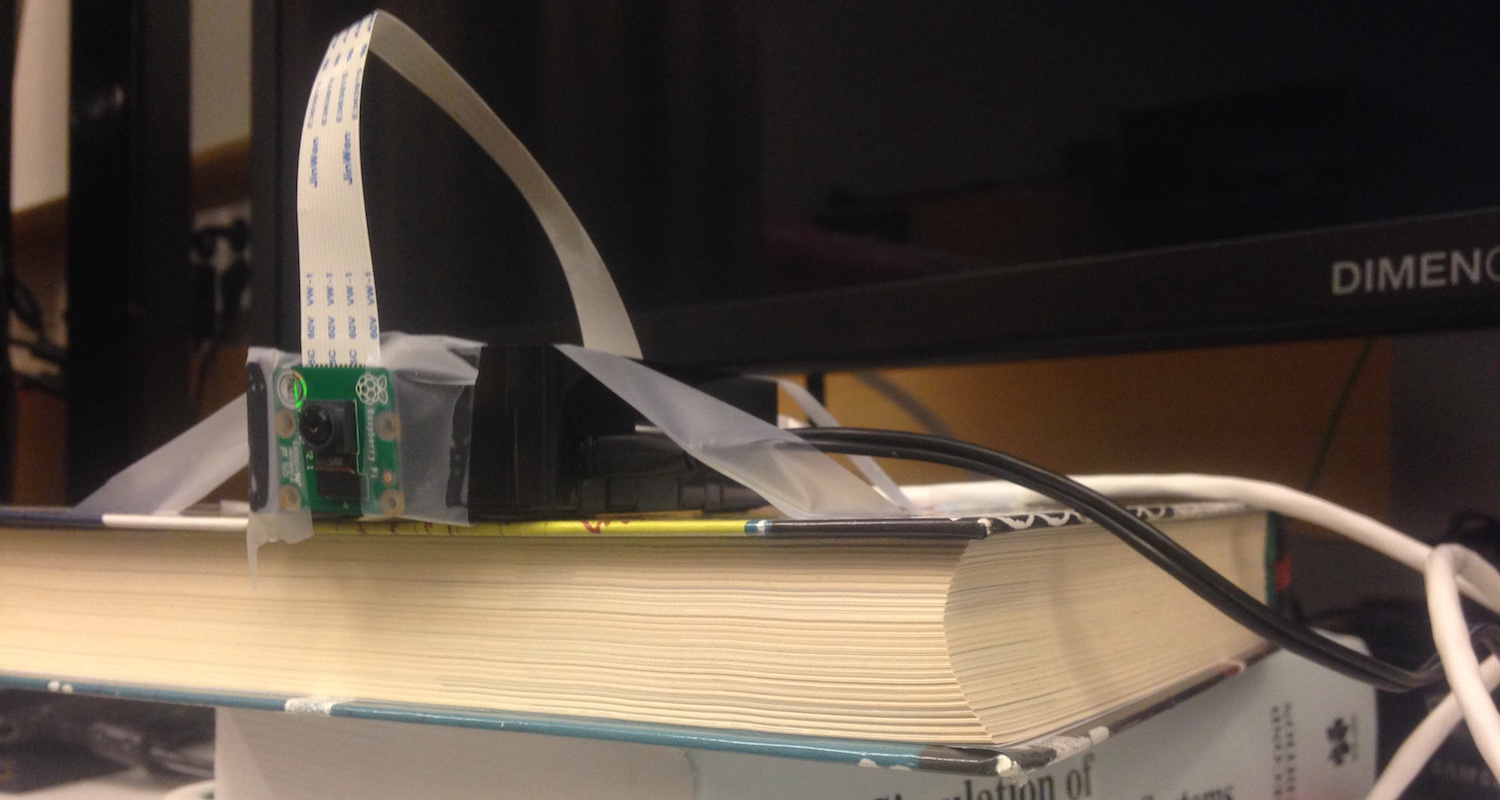
\includegraphics[width=0.49\textwidth]{bin/cameraMount.jpg}} 
	\subfigure[Use barrier to stabilize]{
		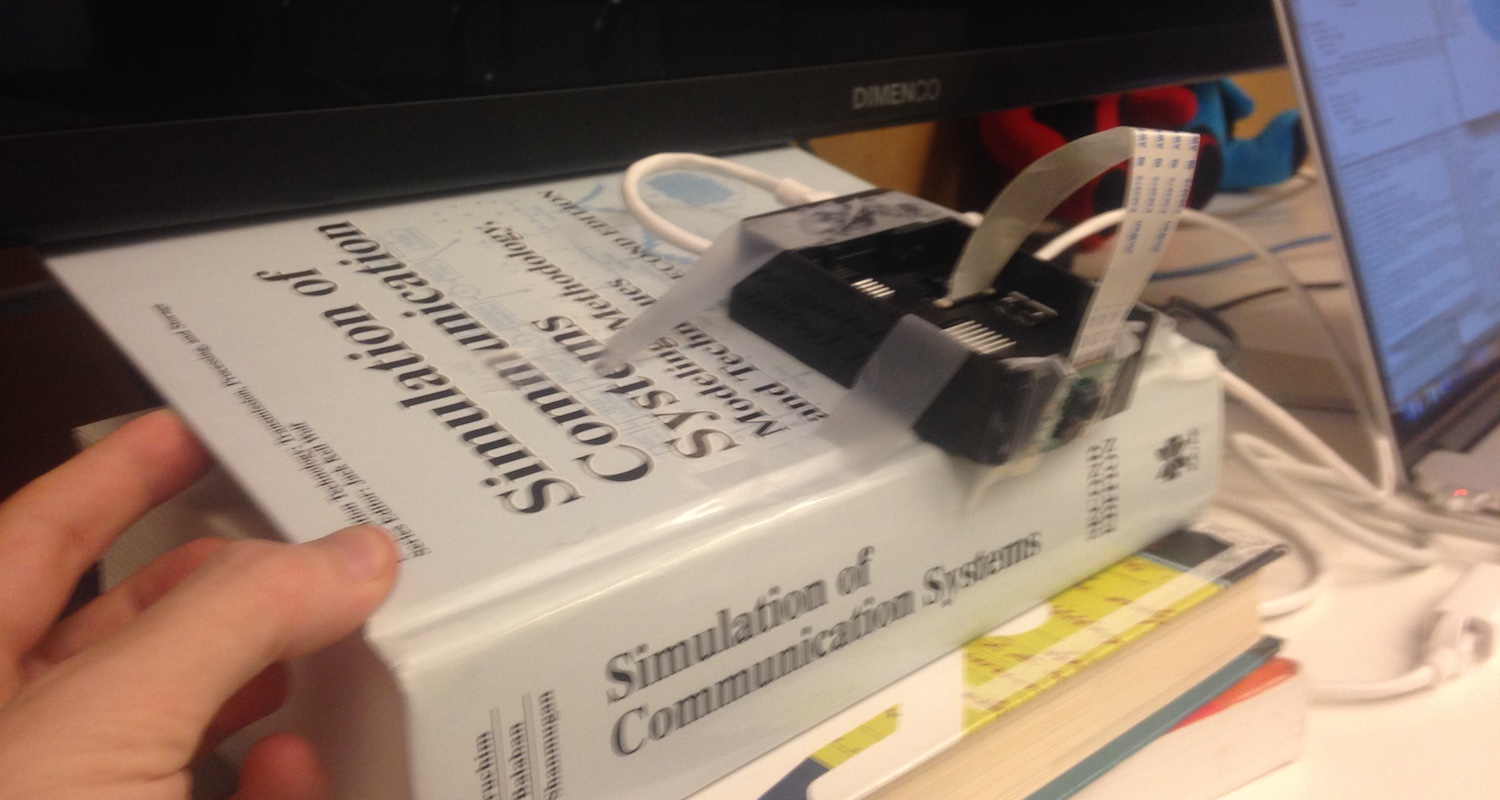
\includegraphics[width=0.49\textwidth]{bin/cameraBarrier.jpg}} 
	\caption{Capturing test sequences} 
	\label{fig:capture}
\end{figure} 
 
To provide meaningful percentage values of missed changes, all changes were executed exactly 100 times for each sequence. 
 
 
 \section{Generate statistics data}
 \label{sec:measurement}
 The data used in the diagrams in the chapter "Results" is generated within a pipeline inside the gstreamer-plugin. In order to produce analytic data, the MIUN\_ANALYTIC precompiler variable has to be set to a non-zero value. Afterwards it produces the following files inside the \enquote{/gstreamer} folder:
 \begin{description}
 	\item[matches.data] 
 	Each row represents one image in the test sequence. The columns contain the following values:
 	\begin{enumerate}
 		\item{Frameindex}
 		\item{Number of corners found}
 		\item{Number of corners expected}
 		\item{Difference between courners found and expected}
 	\end{enumerate}
 	\item[poi.data] 
 	Contains the coordinates of all POIs for each image and weather they are still considered to be corners on that particular image.
 	\begin{enumerate}
 		\item{Position X}
 		\item{Position Y}
 		\item{1 if still a corner, 0 if not a corner anymore}
 	\end{enumerate}
 	
 	\item[changes.data] 
 	Each row in that file represents a change which consists of a startframeindex and a endframeindex. This data is used to benchmark the algorithm.
 \end{description}
 \pagebreak
 For visual feedback, the following command transforms the raw video data into enumerated jpg-images which can easily be inspected in a image-browser. 
 
 \begin{lstlisting}[language=bash]
 docker-compose run gstreamer gst-launch-1.0 \
 filesrc location=data/raw/camVertMove.yuv \
 ! videoparse width=1280 height=720 format=2 \
 ! jpegenc \
 ! multifilesink location=data/sequence/verticalMove/im%06d.jpg
 \end{lstlisting}
 
\chapter{Algorithm design}

\section{Overview}
In the beginning, an entire image is scanned to find prominent pixels, whose coordinates are stored in a vector $\vec{p}$. In the following images, the algorithm just calculates these specific points and checks if they are still considered to be prominent. If too many points are not prominent anymore, a changeStart event is triggered and the $\vec{p}$ is recalculated. When the number of prominent pixel stabilizes in subsequent images, a changeStop event is fired.

\section{Finding pixels of interest}
To find the pixels of interest $\vec{p}$, the entire image is scanned with an algorithm inspired by Harris edge filter. Because of the problem described in section~\ref{sec:harris}, the image is split horizontally and vertically into a configurable amount of subsections  (fig. 5.1), instead of using local maximums to detect the corners. Each subsection is scanned for it's biggest corner-value. Thereby, each corner becomes responsible for its surrounding area in the image and a upper bound of impact could be given for each subsection. 

$$ 1 / nrOfSubsectionsWithCorner $$

If the maximum value inside of a subsection exceeds a predefined threshold, a tuple of that value and the pixel coordinates is stored into $\vec{p}$. The threshold is importent because areas without any visible edges shouldn't affect the result.

\begin{figure}[h!]
	\centering
	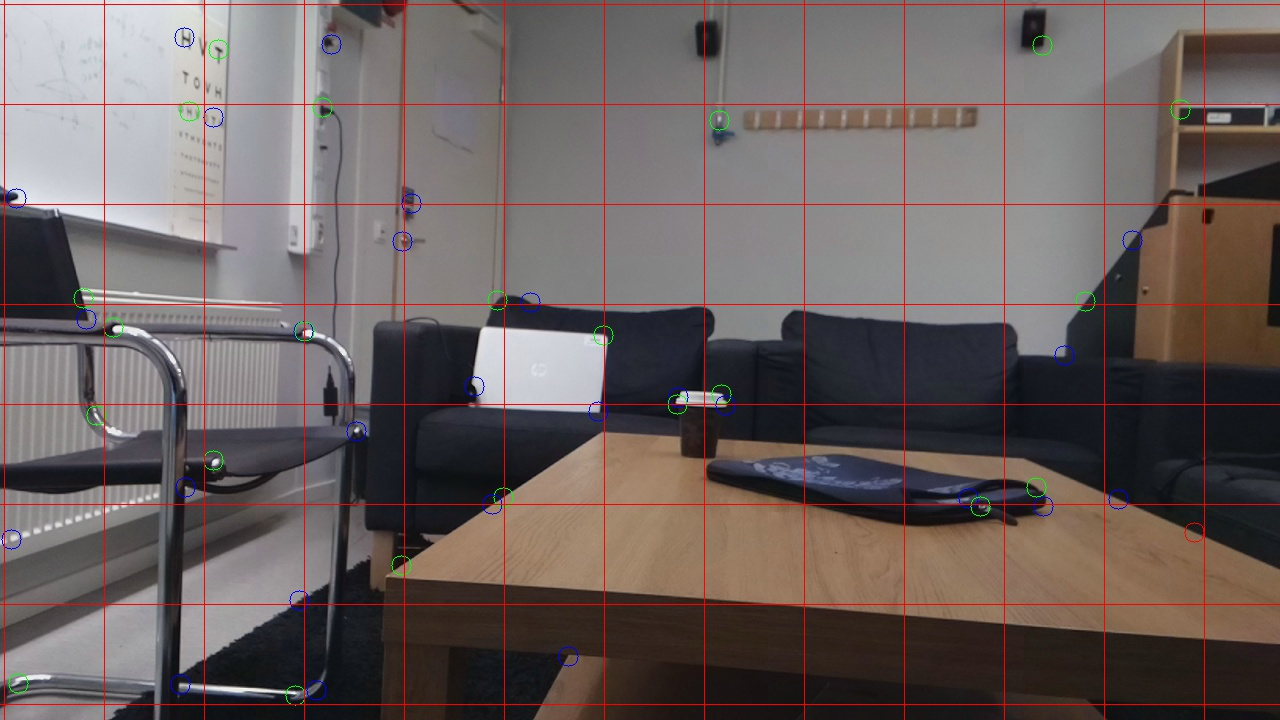
\includegraphics[width=0.9\linewidth]{bin/hotspots}
	\caption{Camera image with a overlay of found edges in each subsection. The red circle in the right bottom represents a point which isn't considered to be an edge anymore. }
	\label{fig:hotspots}
\end{figure} 

\section{ Check pixels of interest}
In subsequent images, just the coordinates stored in $\vec{p}$ are calculated.  For each tuple in the vector (e.g. x,y,value) newValue is determined in the new image at position x:y. When newValue is relatively big enough compared to the value stored in the tuple, the point which the touple represents is still considered to be a corner. This relative solution results in less noise then when comparing it again to the threshold used when the vector is built, because values close to the threshold were toggling to be a corner or not in some frames. Furthermoore, neighbour pixels of very strong edges were still considered to be edges, even though the image moved slightly. 

If the amount of missing corners becomes bigger than a 50\% of |$\vec{p}$|, a changeStart is triggered.

\section{ Stabilize}
In the last phase, the algorithm waits untill the number of found edges stops changing for 3 Frames in a row ($\pm$ 1 corner tolerance). During this phase the vector might be recalculated as well if there are not enough matches.



\chapter{Technical decisions}
\section{Halide}
Because the same algorithm must run over the entire image in the first place and afterwards over specific pixels only, it is important that the  algorithm could handle both tasks in order to avoid the effort of programming everything twice and, more imprtant, assure that it always has the same result. 

Halide allows to write optimized code for both scenarios by separating the algorithm from the schedule \cite{halide}.

\section{32 Bit Kernel}
Even though the Raspberry PI 3 has a 64bit processor, at the time of writing, there are no mature linux distributions for the raspberry with a 64bit kernel out there. As soon as they're available, switching to a 64Bit kernel is higly recommended to allow halide to take advantage of many additional CPU-registers to enhance the performance.


\chapter {Technical implementation}

\section{ Docker }
This project uses docker, a lightwight container virtualization solution, to develop and test the quality of the algorithms. All images used in this project are published on hub.docker.com. Because they are autobuilt, which means that hub.docker.com builds them out of so called Dockerfiles, you can reliably see, how these images are set up. When docker is properly installed, the following commands will download all required files if they is not available locally.

\section{Build process}
All required files are available under \enquote{https://github.com/mineichen/cameraChangeDetection}. The build process is split into two phases and is not fully automated yet.
 
\begin{enumerate}
	\item{ Generate the harris-filter as a static C library}
	\item{ Compile the GStreamer plugin as a dynamic C library}
\end{enumerate}

In order to execute the build commands, the current working directory has to be the same as the project root directory.

\subsection{Harris-Filter}
The Harris-filter is build with the halide programming language. Because halide comes with a cross-compiler built in, the harris binaries for the development-platform and the raspberry pi are compiled inside of a halide-docker-container. The resulting static library inside build/*platform* doesn't have any dependencies to halide. To change the target platform, the \enquote{platform}-variable in halide/build.sh has to be changed.

\begin{lstlisting}[language=bash]
$ docker-compose run halide sh code/build.sh
\end{lstlisting}

For development purpose, the precompiler-condition in the main function could be changed to apply the algorithm to a single png image. 

\subsection{Gstreamer-Plugin}
To create the structure of the plugin, the tool gst-element-maker was used \cite{element-maker}. Unlike the Harris filter, the Gstreamer-Plugin isn't prepared to be cross compiled. Therefore, the compilation is done on the target platform by executing the \enquote{gstreamer/build.sh} script. For development purpose, the following command builds the dynamic-library, which has to be linked to gst-launch at runtime.

\begin{lstlisting}[language=bash]
docker-compose run gstreamer sh code/build.sh
\end{lstlisting}

The static Harris-filter-library has to be copied into the gstreamer/lib/ folder to be found by the compiler. \enquote{gstreamer/codes.txt} contains useful gst-launch pipelines with examples.

\chapter{Results}
In this chapter, the performances of the algorithm using data generated as described in section \ref{sec:measurement} for all captured  scenes defined in section \ref{sec:sequences} is visualized. The red line in the diagrams represents the amount of corners expected to be found and the blue line represents the amount of corners actually found in each frame. During the analysis, the parameter which determines, which percentage of the original cornervalue a subsequent corner has to met, to be considered a corner, had a big influence in the result. Therefore the following sections contain the result with the parameters 50\% on top and 75\% on the bottom. The red areas represent the timespan between changeStart and changeEnd events.

\section{Bump}
The algorithm hasn't missed a single bump or triggered one when there was any. Therefore the project goals G1+G2 are fulfilled.

\begin{tikzpicture}
	\begin{axis}[
          width=\linewidth, % Scale the plot to \linewidth
          height=200,
          grid=major, % Display a grid
          grid style={dashed,gray!30}, % Set the style
          xlabel=Framenumber, % Set the labels
          ylabel=Nr. of matching points,
          %x unit=\si{\volt}, % Set the respective units
          %y unit=\si{\ampere},
          legend style={at={(0.5,-0.2)},anchor=north}, % Put the legend below the plot
          x tick label style={anchor=north,yshift=-2}, % Display labels sideways
          y tick label style={anchor=east,xshift=-2},
          ymin=0,
          xmin=0,
          xmax=200
        ]
		\addplot table [x=frame,y=points, col sep=comma	] {data/bump/final.csv};
		\addplot table [x=frame, y=total, col sep=comma] {data/bump/final.csv};
	\end{axis}
\end{tikzpicture}

\begin{tikzpicture}
\begin{axis}[
width=\linewidth, % Scale the plot to \linewidth
height=200,
grid=major, % Display a grid
grid style={dashed,gray!30}, % Set the style
xlabel=Framenumber, % Set the labels
ylabel=Nr. of matching points,
%x unit=\si{\volt}, % Set the respective units
%y unit=\si{\ampere},
legend style={at={(0.5,-0.2)},anchor=north}, % Put the legend below the plot
x tick label style={anchor=north,yshift=-2}, % Display labels sideways
y tick label style={anchor=east,xshift=-2},
ymin=0,
xmin=0,
xmax=200
]
\addplot+[
	emphasize=8:11 with red!10,
	emphasize=24:35 with red!10,
	emphasize=41:45 with red!10,
	emphasize=59:65 with red!10,
	emphasize=78:83 with red!10,
	emphasize=93:99 with red!10,
	emphasize=107:116 with red!10,
	emphasize=121:127 with red!10,
	emphasize=135:140 with red!10,
	emphasize=148:155 with red!10,
	emphasize=161:167 with red!10,
	emphasize=175:181 with red!10,
	emphasize=188:193 with red!10,
	emphasize=202:212 with red!10,
] table [x=frame, y=points, col sep=comma] {data/bump/final3div4.csv};
\addplot table [x=frame, y=total, col sep=comma] {data/bump/final3div4.csv};
\end{axis}
\end{tikzpicture}

\section{ChangeScene}
In that sequence, there was no change triggered. The lowest amount of matching points was reached in frame 630, where the chair was moved which held many POIs in the scene. The black notebook-bag was moved permanently in frame number 470. 

This shows, that the algorithm has a weakness for permanent changes in the scene. If too many of these happen, a change will trigger even though the camera didn't move. 

Despite a change was almost triggered in frame 630 (fig. 8.1), there was no false positive and no false negative (G1 + G2 achieved).

\begin{tikzpicture}
	\begin{axis}[
          width=\linewidth, % Scale the plot to \linewidth
          height=200,
          grid=major, % Display a grid
          grid style={dashed,gray!30}, % Set the style
          xlabel=Framenumber, % Set the labels
          ylabel=Nr. of matching points,
          %x unit=\si{\volt}, % Set the respective units
          %y unit=\si{\ampere},
          legend style={at={(0.5,-0.2)},anchor=north}, % Put the legend below the plot
          x tick label style={anchor=north,yshift=-2}, % Display labels sideways
          y tick label style={anchor=east,xshift=-2},
          ymin=0,
          xmin=0,
          xmax=1500
        ]
		\addplot table [x=frame, y=points, col sep=comma] {data/sceneChange/final.csv};
		\addplot table [x=frame, y=total, col sep=comma] {data/sceneChange/final.csv};
	\end{axis}
\end{tikzpicture}


\begin{tikzpicture}
\begin{axis}[
width=\linewidth, % Scale the plot to \linewidth
height=200,
grid=major, % Display a grid
grid style={dashed,gray!30}, % Set the style
xlabel=Framenumber, % Set the labels
ylabel=Nr. of matching points,
%x unit=\si{\volt}, % Set the respective units
%y unit=\si{\ampere},
legend style={at={(0.5,-0.2)},anchor=north}, % Put the legend below the plot
x tick label style={anchor=north,yshift=-2}, % Display labels sideways
y tick label style={anchor=east,xshift=-2},
ymin=0,
xmin=0,
xmax=1500
]
\addplot table [x=frame, y=points, col sep=comma] {data/sceneChange/final3div4.csv};
\addplot table [x=frame, y=total, col sep=comma] {data/sceneChange/final3div4.csv};
\end{axis}
\end{tikzpicture}

\begin{figure}[h!]
	\centering
	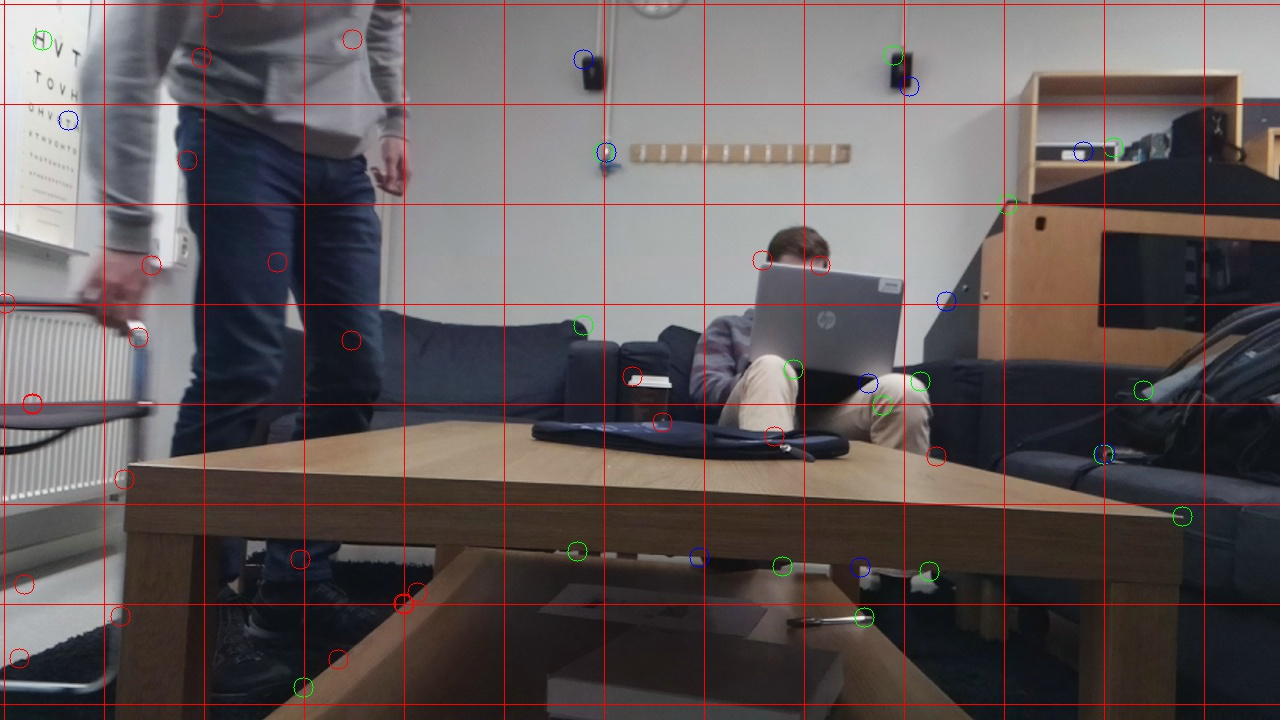
\includegraphics[width=0.9\linewidth]{bin/changeSceneWorst}
	\caption{Worst performance in changeScene sequence. Red Circle means not found anymore. Green and blue is used in a chess-like pattern to distinguish to which subsection a circle belongs to.}
	\label{fig:hotspots}
\end{figure} 
\pagebreak 

\section{NoChange}
The following diagrams show that the algorithm doesn't trigger any unnecessary changes if the scene is not changed and the camera not touched.

\begin{tikzpicture}
	\begin{axis}[
          width=\linewidth, % Scale the plot to \linewidth
          height=200,
          grid=major, % Display a grid
          grid style={dashed,gray!30}, % Set the style
          xlabel=Framenumber, % Set the labels
          ylabel=Nr. of matching points,
          %x unit=\si{\volt}, % Set the respective units
          %y unit=\si{\ampere},
          legend style={at={(0.5,-0.2)},anchor=north}, % Put the legend below the plot
          x tick label style={anchor=north,yshift=-2}, % Display labels sideways
          y tick label style={anchor=east,xshift=-2},
          ymin=0,
          xmin=0,
          xmax=1500
        ]
		\addplot table [x=frame, y=points, col sep=comma] {data/noChange/final.csv};
		\addplot table [x=frame, y=total, col sep=comma] {data/noChange/final.csv};
	\end{axis}
\end{tikzpicture}

\begin{tikzpicture}
\begin{axis}[
width=\linewidth, % Scale the plot to \linewidth
height=200,
grid=major, % Display a grid
grid style={dashed,gray!30}, % Set the style
xlabel=Framenumber, % Set the labels
ylabel=Nr. of matching points,
%x unit=\si{\volt}, % Set the respective units
%y unit=\si{\ampere},
legend style={at={(0.5,-0.2)},anchor=north}, % Put the legend below the plot
x tick label style={anchor=north,yshift=-2}, % Display labels sideways
y tick label style={anchor=east,xshift=-2},
ymin=0,
xmin=0,
xmax=1500
]
\addplot table [x=frame, y=points, col sep=comma] {data/noChange/final3div4.csv};
\addplot table [x=frame, y=total, col sep=comma] {data/noChange/final3div4.csv};
\end{axis}
\end{tikzpicture}

\pagebreak 
\section{ChangeHorizontal}
Because of the recording technique, this sequence contains not only horizontal, but also rotation movements. Somethimes there is no time to stabilize which leads to very long timeintervals between startChange and endChange events.

12 times the pause between the movements was too short and/or bumpy so that two movements were considered to be one long movement. There was no change which happened not in between a startChange and endChange event. 

At index 508, the algorithm triggered a movement which wasn't one. But 1 false positive out of 1547 frames is still under the threshold of 1\% and the project goals G1+G2 are therefore fulfilled in this sequence as well.

\begin{tikzpicture}
\begin{axis}[
width=\linewidth, % Scale the plot to \linewidth
height=200,
grid=major, % Display a grid
grid style={dashed,gray!30}, % Set the style
xlabel=Framenumber, % Set the labels
ylabel=Nr. of matching points,
%x unit=\si{\volt}, % Set the respective units
%y unit=\si{\ampere},
legend style={at={(0.5,-0.2)},anchor=north}, % Put the legend below the plot
x tick label style={anchor=north,yshift=-2}, % Display labels sideways
y tick label style={anchor=east,xshift=-2},
ymin=0,
xmin=0,
xmax=100
]
\addplot table [x=frame, y=points, col sep=comma] {data/horizontalMove/final.csv};
\addplot table [x=frame, y=total, col sep=comma] {data/horizontalMove/final.csv};
\end{axis}
\end{tikzpicture}

	
\begin{tikzpicture}
\begin{axis}[
width=\linewidth, % Scale the plot to \linewidth
height=200,
grid=major, % Display a grid
grid style={dashed,gray!30}, % Set the style
xlabel=Framenumber, % Set the labels
ylabel=Nr. of matching points,
%x unit=\si{\volt}, % Set the respective units
%y unit=\si{\ampere},
legend style={at={(0.5,-0.2)},anchor=north}, % Put the legend below the plot
x tick label style={anchor=north,yshift=-2}, % Display labels sideways
y tick label style={anchor=east,xshift=-2},
ymin=0,
xmin=0,
xmax=100
]
\addplot+[
	emphasize=1:8 with red!10,
	emphasize=14:20 with red!10,
	emphasize=32:57 with red!10,
	emphasize=62:72 with red!10,
	emphasize=78:92 with red!10
] table [x=frame, y=points, col sep=comma] {data/horizontalMove/final3div4.csv};
\addplot table [x=frame, y=total, col sep=comma] {data/horizontalMove/final3div4.csv};
\end{axis}
\end{tikzpicture}


\pagebreak 
\section{ChangeVertical}
In this sequence it happens as well that two changes are summarized to one big movement ($~$18 Times). Specially at the end of the sequence, when the pause between the movements becomes smaller. But there was no wrong detection and none happened not in between changeStart and changeEnd events. There was no false Positive in this section. The project goals G1+G2 are fulfilled.

\begin{tikzpicture}
\begin{axis}[
width=\linewidth, % Scale the plot to \linewidth
height=200,
grid=major, % Display a grid
grid style={dashed,gray!30}, % Set the style
xlabel=Framenumber, % Set the labels
ylabel=Nr. of matching points,
%x unit=\si{\volt}, % Set the respective units
%y unit=\si{\ampere},
legend style={at={(0.5,-0.2)},anchor=north}, % Put the legend below the plot
x tick label style={anchor=north,yshift=-2}, % Display labels sideways
y tick label style={anchor=east,xshift=-2},
ymin=0,
xmin=0,
xmax=100
]
\addplot table [x=frame, y=points, col sep=comma] {data/verticalMove/final.csv};
\addplot table [x=frame, y=total, col sep=comma] {data/verticalMove/final.csv};
\end{axis}
\end{tikzpicture}
\begin{tikzpicture}
\begin{axis}[
width=\linewidth, % Scale the plot to \linewidth
height=200,
grid=major, % Display a grid
grid style={dashed,gray!30}, % Set the style
xlabel=Framenumber, % Set the labels
ylabel=Nr. of matching points,
%x unit=\si{\volt}, % Set the respective units
%y unit=\si{\ampere},
legend style={at={(0.5,-0.2)},anchor=north}, % Put the legend below the plot
x tick label style={anchor=north,yshift=-2}, % Display labels sideways
y tick label style={anchor=east,xshift=-2},
ymin=0,
xmin=0,
xmax=100
]
\addplot+[
emphasize=5:14 with red!10,
emphasize=23:30 with red!10,
emphasize=39:48 with red!10,
emphasize=56:69 with red!10,
emphasize=74:83 with red!10,
emphasize=91:99 with red!10
] table [x=frame, y=points, col sep=comma] {data/verticalMove/final3div4.csv};
\addplot table [x=frame, y=total, col sep=comma] {data/verticalMove/final3div4.csv};
\end{axis}
\end{tikzpicture}


\chapter{Conclusion}
The algorithm works very reliably on the tested sequences, because all sequences passed the project goals G1+G2. The algorithm hasn't missed a single change in the test sequences. Gstreamer allows a easy porting onto the raspberry pi, which was tested within the project (G3). The biggest weakness of the algorithm are constant changes in the scene. 

Because of the requirements to have a low false negative rate, the mentioned parameter mentioned in the "Results" chapter sould be 75\%. However, both parameters almost had the same results in this sequences. It just detected the changes one frame earlier sometimes. If tiny changes of the camera shouldn't trigger a change event, a lower percentage should be choosen.

The halide programming language works great on the raspberry pi. The separation of schedule and algorithm allows to optimize the code without accidentaly changing the logic. The source code is very easy to understand. 

\chapter{Outlook}
The following sections suggest further studies about the algorithm. Beside mentioning the possible weakness, ideas for a solution of these problems is provided. 

\section{Light changes}
Because the algorithm operates on the corner-values, it shouldn't be vulnerable to small light changes. If lightchanges cause unwanted change events, the algorithm might be extended to operate on the color images of YUV instead of the grayscale image. 

\section{Moving objects in the scene}
The sequence changeScene covered in this project didn't contain the constantly moving objects (e.g. a walking person)  during the step of finding the points of interest $\vec{p} $. If these objects are in the scene from the begining on, the error is bigger because despite the fact that these objects cover other corners, the corners caused by these objects  will not be there anymore.

As a possible solution corners inside $\vec{p} $ could become moore or less weighted depending on how many times they are found in subsequent images.
\chapter{Glossary}
\begin{description}
	\item[MIUN] Mid Sweden university
	\item[YUV] Color format which represents a grayscale image in Y and the color information in UV.
	\item[POI] Point of Interest
	\item[Scene] Objects which appear in the recording
	\item[gst] 	Abbreviation for Gstreamer, a streaming framework.
\end{description}
